% Do NOT change this "Section" title
% and do NOT add more "Section" level titles.
\section{Implementation}\label{sec:implementation}
The implementation section describes the changes that have been made to the bootloader and PC client to fit the requirements.




% You can use how many "subsections" and "subsubsections" you like.
\subsection{Bootloader}
\subsubsection{EEPROM byte for boot status}
EBSB is a byte created in the EEPROM that determines if the bootloader should run or if the flash program should run. If the byte is set to 255 (0xFF) then it will jump to the flash program. Any other value allows the bootloader to run. This byte changes according to the demands of the PC client and since it is written in the EEPROM the value remains the same, even on reset.

\subsubsection{EEPROM byte for ID}
Each AT90CAN with a bootloader is assigned an ID number between 0 and 255. ENNB is a byte created in the EEPROM that stores the ID of the microcontroller. This makes it possible for the bootloader to identify itself when communicating with the PC client.

\subsubsection{Message to change EBSB}
The bootloader will now listen for one more message. If the bootloader receives a BOOT\_STATUS message with CAN ID 11 then it will change the EEPROM byte EBSB into whatever value was sent in the first byte of the CAN message.

\subsection{Configuration Manager}

\subsubsection{New protocol for sending messages}
The weRobot PC client was designed to be connected directly to the CAN-bus and send CAN messages. However Naiad will connect to the system via the CAN-logger board through an ethernet connection. For this reason it was necessary to replace the CAN protocol with a new protocol using TCP sockets instead. This new ethernet protocol is designed to stream the contents of a CAN message over the ethernet connection and then rebuild it into a CAN message at the receiver. 

For more information on where this is used see step 8 in Figure ~\ref{fig:activity_figure}.

\subsubsection{List of configured nodes}
The PC client has a configuration file named card\_names.cfg. This file matches the ID of different nodes in the system with a name. The PC client will display all these configured nodes in a list. When the user wants any node to enter the bootloader it will first be selected from this list.

For more information on where this is used see step 1 in Figure ~\ref{fig:activity_figure}.

\subsubsection{Button to start bootloader}
The start bootloader button is used to make the node that has been selected in the list of configured nodes to enter the bootloader. The PC client will first send a mode message with CAN ID 380 and the first byte set to 2 for bootloader mode. This is to tell the whole system that one or more nodes are going to be programmed through the bootloader. After waiting a brief moment it will send START\_BOOTLOADER message with CAN ID 12. This message signals to the selected node that it should enter the bootloader. The first byte in this message holds the ID of the node. Once completed it will send a DISCOVER message with CAN ID 7 to which all nodes that has entered the bootloader will respond. The PC client will then display all the discovered nodes that replied.

For more information on where this is used see step 2 in Figure ~\ref{fig:activity_figure}.

\begin{figure}[h]
\begin{center}
    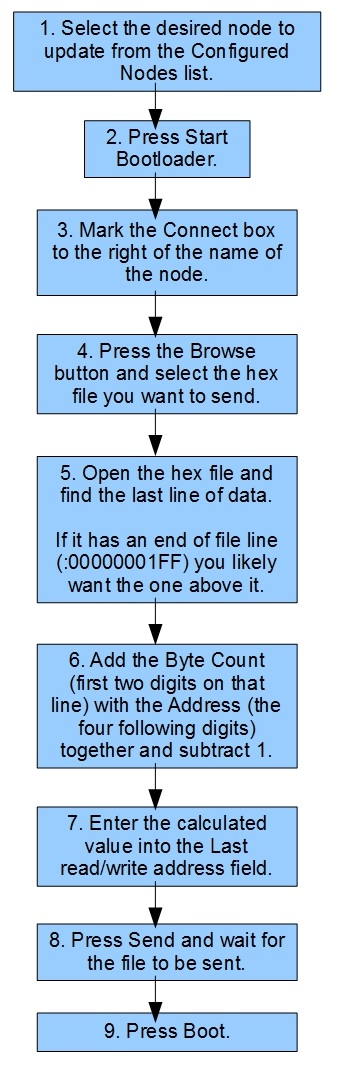
\includegraphics[width=0.20\textwidth]{./figure/activity.jpg}
\end{center}
    \caption{Activity diagram example}
    \label{fig:activity_figure}
\end{figure}